% !TEX TS-program = pdflatex
% !TEX encoding = UTF-8 Unicode

% This is a simple template for a LaTeX document using the "article" class.
% See "book", "report", "letter" for other types of document.

\documentclass[11pt]{article} % use larger type; default would be 10pt

\usepackage[utf8]{inputenc} % set input encoding (not needed with XeLaTeX)

%%% Examples of Article customizations
% These packages are optional, depending whether you want the features they provide.
% See the LaTeX Companion or other references for full information.

%%% PAGE DIMENSIONS
\usepackage{geometry} % to change the page dimensions
\geometry{a4paper} % or letterpaper (US) or a5paper or....
% \geometry{margin=2in} % for example, change the margins to 2 inches all round
% \geometry{landscape} % set up the page for landscape
%   read geometry.pdf for detailed page layout information

\usepackage{graphicx} % support the \includegraphics command and options

% \usepackage[parfill]{parskip} % Activate to begin paragraphs with an empty line rather than an indent

%%% PACKAGES

\usepackage{setspace}
\usepackage{listings}
\usepackage{hyperref}
\hypersetup{
    colorlinks=true,
    linkcolor=blue,
    filecolor=magenta,      
    urlcolor=cyan,
}

\usepackage{color}

\definecolor{dkgreen}{rgb}{0,0.6,0}
\definecolor{gray}{rgb}{0.5,0.5,0.5}
\definecolor{mauve}{rgb}{0.58,0,0.82}

\lstset{frame=L,
  language=Python,
  aboveskip=3mm,
  belowskip=3mm,
  showstringspaces=false,
  columns=flexible,
  basicstyle={\small\ttfamily},
  numbers=none,
  numberstyle=\tiny\color{gray},
  keywordstyle=\color{blue},
  commentstyle=\color{dkgreen},
  stringstyle=\color{mauve},
  breaklines=true,
  breakatwhitespace=true,
  tabsize=3
}

\usepackage{booktabs} % for much better looking tables
\usepackage{array} % for better arrays (eg matrices) in maths
\usepackage{paralist} % very flexible & customisable lists (eg. enumerate/itemize, etc.)
\usepackage{verbatim} % adds environment for commenting out blocks of text & for better verbatim
\usepackage{subfig} % make it possible to include more than one captioned figure/table in a single float
% These packages are all incorporated in the memoir class to one degree or another...

%%% HEADERS & FOOTERS
\usepackage{fancyhdr} % This should be set AFTER setting up the page geometry
\pagestyle{fancy} % options: empty , plain , fancy
\renewcommand{\headrulewidth}{0pt} % customise the layout...
\lhead{}\chead{}\rhead{}
\lfoot{}\cfoot{\thepage}\rfoot{}

%%% SECTION TITLE APPEARANCE
\usepackage{sectsty}
\allsectionsfont{\sffamily\mdseries\upshape} % (See the fntguide.pdf for font help)
% (This matches ConTeXt defaults)

%%% ToC (table of contents) APPEARANCE
\usepackage[nottoc,notlof,notlot]{tocbibind} % Put the bibliography in the ToC
\usepackage[titles,subfigure]{tocloft} % Alter the style of the Table of Contents
\renewcommand{\cftsecfont}{\rmfamily\mdseries\upshape}
\renewcommand{\cftsecpagefont}{\rmfamily\mdseries\upshape} % No bold!
\graphicspath{ {../images/} }


%%% END Article customizations

%%% The "real" document content comes below...

\title{Zomato Restaurants Data Analysis}
\author{
Mateja Marjanović\\
\texttt{172/2015}
}
%\date{} % Activate to display a given date or no date (if empty),
         % otherwise the current date is printed 

\begin{document}
\pagenumbering{gobble}
\maketitle
\newpage

\doublespacing
\tableofcontents
\singlespacing
\newpage

\pagenumbering{arabic}

\section{Uvod}
Podaci su skinuti na linku \url{https://www.kaggle.com/shrutimehta/zomato-restaurants-data}. Podaci se nalaze u datotekama: zomato.csv i Country-Code.xlsx i u njima se nalaze informacije o restoranima i mapa koji kod se slika u koju drzavu. Ostali podaci ce biti ili generisani na osnovu tih ili jos i uz pomoc biblioteke
BeautifulSoup koja ce da povlaci sa raznih stranica na internetu.

\section{Analiza i pretprocesiranje podataka}
U datoteci Country-Code ima samo dve kolone, to su ime drzave i kod koji se koristi u datoteci zomato koji predstavlja drzavu u kojoj se nalazi restoran. Opisi kolona datoteke zomato.csv su dati u tabeli 1.
\newline\newline
\begin{tabular}{|l|l|}
\hline
Restaurant Id & jedinstveni identifikator restorana \\
\hline
Restaurant Name & ime restorana \\
\hline
Country Code & celobrojna vrednost koja predstavlja kod drzave \\
\hline
City & ime grada u kome se nalazi restoran \\
\hline
Adress & adresa restorana \\
\hline
Locality & lokacija restorana \\
\hline
Locality Verbose & detaljno opisana lokacija restorana\\
\hline
Longitude & geografska duzina \\
\hline
Latitude & geografska sirina \\
\hline
Cuisines & kuhinje koje restoran nudi \\
\hline
Average Cost for two & prosecna cena za dvoje izrazena u razlicitim valutama \\
\hline
Currency & valuta koja se koristi \\
\hline
Has Table booking & da/ne \\
\hline
Has Online delivery & da/ne \\
\hline
Is delivering now & da/ne \\
\hline
Switch to order menu & da/ne \\
\hline
Price range & raspon cena \\
\hline
Aggregate rating & prikupljena procena \\
\hline
Rating color & boja procene \\
\hline
Rating text & tekst procene \\
\hline
Votes & broj glasova od ljudi \\
\hline
\end{tabular}

\subsection{Analiza podataka}
Pogledajmo detaljnije nasu datoteku. Koristimo Python kod da izlistamo osnovne informacije o podacima.
Pre nego sto pocnemo uradimo odmah zamenu kolone Country Code sa kolonom Country.
\begin{lstlisting}
import xlrd
import pandas as pd

dfRestaurants = pd.read_csv("zomato.csv", encoding = "ISO-8859-1")
dfCountries = pd.read_excel('Country-Code.xlsx', sheetname="Sheet1", index_col = "Country Code")

countriesData = []
for i, row in dfRestaurants.iterrows():
    countryCode = int(row["Country Code"])
    countriesData.append(dfCountries.ix[countryCode]["Country"])

dfRestaurants["Country"] = pd.Series(countriesData, index = dfRestaurants.index)
dfRestaurants = dfRestaurants.drop(["Country Code"], axis = 1)

with open("zomatoCountryAdded.csv", "w") as csvFile:
    csv = dfRestaurants.to_csv(index = True)
    csvFile.write(csv)
\end{lstlisting}
Sada necemo koristiti vise datoteku zomato.csv, vec zomatoCountryAdded.csv.
\begin{lstlisting}
import pandas as pd
print("***********", "*zomatoCountryAdded.csv*", "***********", "\n", sep="\n")

df_restaurants = pd.read_csv("zomatoMissingValuesRemoved.csv")
print(df_restaurants.head(), "\n")
print(df_restaurants.count(), "\n")
print(df_restaurants.describe(), "\n")
for column in df_restaurants.columns:
    print("Count values in column " + column, "\n")
    print(df_restaurants[column].value_counts(dropna=False))

\end{lstlisting}
rezultat izvrsavanja:
\begin{lstlisting}
************************
*zomatoCountryAdded.csv*
************************

   Restaurant ID         Restaurant Name              City  \
0        6317637        Le Petit Souffle       Makati City   
1        6304287        Izakaya Kikufuji       Makati City   
2        6300002  Heat - Edsa Shangri-La  Mandaluyong City   
3        6318506                    Ooma  Mandaluyong City   
4        6314302             Sambo Kojin  Mandaluyong City   

                                             Address  \
0  Third Floor, Century City Mall, Kalayaan Avenu...   
1  Little Tokyo, 2277 Chino Roces Avenue, Legaspi...   
2  Edsa Shangri-La, 1 Garden Way, Ortigas, Mandal...   
3  Third Floor, Mega Fashion Hall, SM Megamall, O...   
4  Third Floor, Mega Atrium, SM Megamall, Ortigas...   

                                     Locality  \
0   Century City Mall, Poblacion, Makati City   
1  Little Tokyo, Legaspi Village, Makati City   
2  Edsa Shangri-La, Ortigas, Mandaluyong City   
3      SM Megamall, Ortigas, Mandaluyong City   
4      SM Megamall, Ortigas, Mandaluyong City   

                                    Locality Verbose   Longitude   Latitude  \
0  Century City Mall, Poblacion, Makati City, Mak...  121.027535  14.565443   
1  Little Tokyo, Legaspi Village, Makati City, Ma...  121.014101  14.553708   
2  Edsa Shangri-La, Ortigas, Mandaluyong City, Ma...  121.056831  14.581404   
3  SM Megamall, Ortigas, Mandaluyong City, Mandal...  121.056475  14.585318   
4  SM Megamall, Ortigas, Mandaluyong City, Mandal...  121.057508  14.584450   

                           Cuisines  Average Cost for two     ...       \
0        French, Japanese, Desserts                  1100     ...        
1                          Japanese                  1200     ...        
2  Seafood, Asian, Filipino, Indian                  4000     ...        
3                   Japanese, Sushi                  1500     ...        
4                  Japanese, Korean                  1500     ...        

  Has Table booking Has Online delivery Is delivering now  \
0               Yes                  No                No   
1               Yes                  No                No   
2               Yes                  No                No   
3                No                  No                No   
4               Yes                  No                No   

  Switch to order menu Price range  Aggregate rating  Rating color  \
0                   No           3               4.8    Dark Green   
1                   No           3               4.5    Dark Green   
2                   No           4               4.4         Green   
3                   No           4               4.9    Dark Green   
4                   No           4               4.8    Dark Green   

  Rating text Votes      Country  
0   Excellent   314  Phillipines  
1   Excellent   591  Phillipines  
2   Very Good   270  Phillipines  
3   Excellent   365  Phillipines  
4   Excellent   229  Phillipines  

[5 rows x 21 columns] 

Restaurant ID           9542
Restaurant Name         9542
City                    9542
Address                 9542
Locality                9542
Locality Verbose        9542
Longitude               9542
Latitude                9542
Cuisines                9542
Average Cost for two    9542
Currency                9542
Has Table booking       9542
Has Online delivery     9542
Is delivering now       9542
Switch to order menu    9542
Price range             9542
Aggregate rating        9542
Rating color            9542
Rating text             9542
Votes                   9542
Country                 9542
dtype: int64 

       Restaurant ID    Longitude     Latitude  Average Cost for two  \
count   9.542000e+03  9542.000000  9542.000000           9542.000000   
mean    9.043301e+06    64.274997    25.848532           1200.326137   
std     8.791967e+06    41.197602    11.010094          16128.743876   
min     5.300000e+01  -157.948486   -41.330428              0.000000   
25%     3.019312e+05    77.081565    28.478658            250.000000   
50%     6.002726e+06    77.192031    28.570444            400.000000   
75%     1.835260e+07    77.282043    28.642711            700.000000   
max     1.850065e+07   174.832089    55.976980         800000.000000   

       Price range  Aggregate rating         Votes  
count  9542.000000       9542.000000   9542.000000  
mean      1.804968          2.665238    156.772060  
std       0.905563          1.516588    430.203324  
min       1.000000          0.000000      0.000000  
25%       1.000000          2.500000      5.000000  
50%       2.000000          3.200000     31.000000  
75%       2.000000          3.700000    130.000000  
max       4.000000          4.900000  10934.000000   

Count values in column Restaurant ID 

2047        1
308620      1
7561        1
18294392    1
...
8913        1
4815        1
3200002     1
18254540    1
18432000    1
Name: Restaurant ID, dtype: int64
Count values in column Restaurant Name 

Cafe Coffee Day                    83
Domino`s Pizza                     79
Subway                             63
Green Chick Chop                   51
McDonald`s                         48
Keventers                          34
Pizza Hut                          30
...
The Bay Leaf                        1
Papa Mexicano                       1
Aapki Apni Rasoi                    1
Mathura Lassi Wala                  1
Bao                                 1
Mittal Restaurant & Fast Food       1
Mukhtalif Biryanis                  1
Sona                                1
Lazeez Foods                        1
Name: Restaurant Name, dtype: int64
Count values in column City 

New Delhi                 5473
Gurgaon                   1118
Noida                     1080
Faridabad                  251
Ghaziabad                   25
Bhubaneshwar                21
Amritsar                    21
Ahmedabad                   21
Lucknow                     21
Guwahati                    21
Mumbai                      20
Pocatello                   20
Kanpur                      20
Surat                       20
Doha                        20
Cedar Rapids/Iowa City      20
...
Phillip Island               1
Vernonia                     1
Randburg                     1
Inverloch                    1
Victor Harbor                1
Princeton                    1
Forrest                      1
Quezon City                  1
Paynesville                  1
Ojo Caliente                 1
Potrero                      1
Mohali                       1
Name: City, dtype: int64
Count values in column Address 

Dilli Haat, INA, New Delhi                                                               11
Sector 41, Noida                                                                         11
Greater Kailash (GK) 1, New Delhi                                                        10
The Imperial, Janpath, New Delhi                                                          9
HUDA Market, Sector 56, Gurgaon                                                           8
Food Court, 3rd Floor, Logix City Centre, Sector 32, Near Sector 34, Noida                8
Palate of Delhi, Dhaula Kuan Metro Station, Chanakyapuri, New Delhi                       8
Cyber Hub, DLF Cyber City, Gurgaon                                                        8
The Lalit, Barakhamba Avenue, Barakhamba Road, New Delhi                                  8
The Taj Mahal Hotel, 1, Mansingh Road, New Delhi                                          7
DLF Phase 1, Gurgaon                                                                      7
Main Market, Ghitorni, MG Road, New Delhi                                                 7
...
223, Moments Mall, Kirti Nagar, New Delhi                                                 1
400 Quietwater Beach Rd, Pensacola Beach, FL 32561                                        1
Shop 4, 25/6, Ground Floor, East Patel Nagar, New Delhi                                   1
Ground Floor, New Delhi Metro Station, Paharganj, New Delhi                               1
10, Sector 1 Market, R K Puram, New Delhi                                                 1
Shop G-11, Aditya Complex, KP Block, Pitampura, New Delhi                                 1
2932 Warm Springs Rd, Columbus, GA 31909                                                  1
P-4, Circular Road, New Colony, Old Railway Road, Gurgaon                                 1
1st Floor, P-13/A, Aacharya Niketan Market, Mayur Vihar Phase 1, New Delhi                1
SCF 74, Sector 15 Market, Sector 15, Faridabad                                            1
22, New Market, Malviya Nagar, New Delhi                                                  1
Name: Address, dtype: int64
Count values in column Locality 

Connaught Place                         122
Rajouri Garden                           99
Shahdara                                 87
Defence Colony                           86
Malviya Nagar                            85
Pitampura                                85
Mayur Vihar Phase 1                      84
Rajinder Nagar                           81
Safdarjung                               80
Satyaniketan                             79
Krishna Nagar                            77
Karol Bagh                               76
Sector 62                                76
...
Bryanston Shopping Centre, Bryanston      1
KadÛ±kí_y Merkez                          1
Cavendish Square, Claremont               1
Sylvester                                 1
Dikmen                                    1
Name: Locality, dtype: int64
Count values in column Locality Verbose 

Connaught Place, New Delhi                                 122
Rajouri Garden, New Delhi                                   99
Shahdara, New Delhi                                         87
Defence Colony, New Delhi                                   86
Pitampura, New Delhi                                        85
Mayur Vihar Phase 1, New Delhi                              84
Malviya Nagar, New Delhi                                    84
Rajinder Nagar, New Delhi                                   81
Safdarjung, New Delhi                                       80
Satyaniketan, New Delhi                                     79
Krishna Nagar, New Delhi                                    76
...
Haji Lane, Rochor, Singapore                                 1
Holiday Inn, Aerocity, New Delhi                             1
Meridian, Boise                                              1
íìmitkí_y, Ankara                                            1
Jukaso It Suites, Sector 14, Gurgaon                         1
Waltair Uplands, Vizag                                       1
Kailua Kona, Rest of Hawaii                                  1
Z Square Mall, Mall Road, Kanpur                             1
Arya Nagar, Kanpur                                           1
Al Barari, Dubai                                             1
Dr. Zakir Hussain Marg, New Delhi                            1
Name: Locality Verbose, dtype: int64
Count values in column Cuisines 

North Indian                                                           936
North Indian, Chinese                                                  511
Fast Food                                                              354
Chinese                                                                354
North Indian, Mughlai                                                  334
Cafe                                                                   299
Bakery                                                                 218
North Indian, Mughlai, Chinese                                         197
Bakery, Desserts                                                       170
Street Food                                                            149
Pizza, Fast Food                                                       131
Chinese, Fast Food                                                     118
Mithai, Street Food                                                    116
South Indian                                                           112
Bakery, Fast Food                                                      108
Chinese, North Indian                                                  105
...
North Indian, South Indian, Bakery, Italian                              1
Pizza, Italian, Beverages, Desserts                                      1
Cafe, Fast Food, Chinese                                                 1
North Indian, South Indian, Chinese, Street Food, Fast Food, Mithai      1
American, Continental, Italian                                           1
North Indian, Chinese, Mughlai, Italian                                  1
Mexican, American, Tex-Mex                                               1
Cafe, Italian, Continental, Mexican                                      1
Chinese, Sushi, Thai                                                     1
Assamese                                                                 1
Filipino, Japanese, Asian                                                1
Burger, Bar Food, Southern                                               1
Name: Cuisines, dtype: int64
Count values in column Average Cost for two 

500       900
300       897
400       857
200       687
600       652
250       461
350       457
700       403
150       367
100       353
800       347
450       335
1000      281
1500      190
...
3210        1
450000      1
3800        1
3650        1
8000        1
545         1
4800        1
535         1
Name: Average Cost for two, dtype: int64
Count values in column Currency 

Indian Rupees(Rs.)        8652
Dollar($)                  473
Pounds(£)                  80
Emirati Diram(AED)          60
Brazilian Real(R$)          60
Rand(R)                     60
NewZealand($)               40
Turkish Lira(TL)            34
Botswana Pula(P)            22
Indonesian Rupiah(IDR)      21
Sri Lankan Rupee(LKR)       20
Qatari Rial(QR)             20
Name: Currency, dtype: int64
Count values in column Has Table booking 

No     8384
Yes    1158
Name: Has Table booking, dtype: int64
Count values in column Has Online delivery 

No     7091
Yes    2451
Name: Has Online delivery, dtype: int64
Count values in column Is delivering now 

No     9508
Yes      34
Name: Is delivering now, dtype: int64
Count values in column Switch to order menu 

No    9542
Name: Switch to order menu, dtype: int64
Count values in column Price range 

1    4438
2    3113
3    1405
4     586
Name: Price range, dtype: int64
Count values in column Aggregate rating 

0.0    2148
3.2     522
3.1     519
3.4     495
3.3     483
3.5     480
3.0     468
3.6     458
3.7     427
3.8     399
2.9     381
3.9     332
2.8     315
4.1     274
4.0     266
2.7     250
4.2     221
2.6     191
4.3     174
4.4     143
2.5     110
4.5      95
2.4      87
4.6      78
4.9      61
2.3      47
4.7      41
2.2      27
4.8      25
2.1      15
2.0       7
1.9       2
1.8       1
Name: Aggregate rating, dtype: int64
Count values in column Rating color 

Orange        3734
White         2148
Yellow        2096
Green         1078
Dark Green     300
Red            186
Name: Rating color, dtype: int64
Count values in column Rating text 

Average      3734
Not rated    2148
Good         2096
Very Good    1078
Excellent     300
Poor          186
Name: Rating text, dtype: int64
Count values in column Votes 

0       1094
1        483
2        327
3        244
4        207
7        168
5        164
6        154
10       135
8        134
11       123
9        113
14       104
12       100
13        95
...
556        1
2589       1
524        1
508        1
2549       1
476        1
1103       1
468        1
388        1
2333       1
284        1
236        1
2213       1
1887       1
1959       1
Name: Votes, dtype: int64
Count values in column Country 

India             8652
United States      425
United Kingdom      80
South Africa        60
Brazil              60
UAE                 60
New Zealand         40
Turkey              34
Australia           24
Phillipines         22
Indonesia           21
Sri Lanka           20
Qatar               20
Singapore           20
Canada               4
Name: Country, dtype: int64
\end{lstlisting}
Iz ovih rezultata mozemo primetiti vise stvari. Tabela ima tacno 9542 unosa, pri cemu kolona Restaurant ID nema nijednom ponavljanje, postoje restorani sa istim
imenima (slucajnost ili lanac restorana npr. KFC), ubedljivo najvise restorana u tabeli je iz Nju Delhija tj. iz Indije, u koloni Locality Verbose mozemo videti 
da su skoro sve najcesce lokacije u Nju Delhiju, a sve u Indiji. Zbog istog broja instanci u kojima su i geografska sirina i geografska duzina 0.0 moze 
se zakljuciti da to nije stvarno tako vec da nije unesena prava vrednost. Posto smo vec videli da je vecina restorana iz Indije ocekivano je da je i vecina kuhinja
indijskog porekla (ili makar azijskog). Kolonu Average Cost for two necemo trenutno razmatrati, jer su u razlicitim valutama, malo kasnije cemo to sve 
konvertovati u evre pa cemo onda to koristiti. Kolona Currency nam govori o valuti koja se korisi u toj drzavi i skoro je isto kao i kolona Country koju cemo 
tek obraditi. Kolonu Switch to order menu necemo uopste koristiti jer u nasoj tabeli ima iskljucivo vrednost No, pa nam nista ne znaci. Na osnovu kolone 
Price range mozemo videti da je cesce manja vrednost nego veca (cesce 1 nego 4) sto znaci da je uglavnom raspon cena mali u vecini restorana (ako je prosecna
cena za dvoje niska/prosecna/visoka verovatno je to dovoljno dobra pretpostavka). U koloni Aggregate rating vidimo da je veliki broj restorana ocenjen sa 0.0, 
to najverovatnije znaci da nisu ocenjeni, a ne da su mnogo losi. Kolone Rating color i Rating text su redundantne, pa cemo gledati samo Rating text, jer j
e razumljivije. Ocigledno je da ljudi cesce daju prosecne ili dobre ocene pre nego lose, pa zato samo 186 vrednosti je Poor, dok Average, Good i Very Good ima 
mnogo vise. Kolona Votes nam opet govori da ljudi cesto ne glasaju, cak 1094 restorana nema nijedan glas. I na kraju ponovo da potvrdimo da u Indiji ima 
8652 restorana, u Americi 425, dok je u svim ostalim zemljama taj broj dvocifren (ili cak jednocifren).

U KNIME-u cemo 'ocistiti' nase podatke i eliminisati instance sa nedostajucim vrednostima (koristimo cvor Missing Values).

\subsection{Analiza pojedinacnih kolona}
Prva stvar koju cemo uraditi je pokrenuti par skriptova koji ce na osnovu nase tabele i jos nekih tabela ciji su podaci prikupljeni zasebno, generisati neke 
nove kolone.
\subsubsection{Prosecna plata u drzavama}
Na linku \url{"http://www.nationmaster.com/country-info/stats/Cost-of-living/Average-monthly-disposable-salary/After-tax} se nalazi tabela sa imenom drzave 
i prosecnom platom u toj drzavi. Koristeci biblioteku BeautifulSoup povukli smo sa te stranice te podatke i smestili ih u fajl countrySalaries.csv. 
\begin{lstlisting}
import pandas as pd
from bs4 import BeautifulSoup as soup
from urllib.request import urlopen as uReq

salariesUrl = "http://www.nationmaster.com/country-info/stats/Cost-of-living/Average-monthly-disposable-salary/After-tax"

uClient = uReq(salariesUrl)
pageHtml = uClient.read()
uClient.close()

pageSoup = soup(pageHtml, "html.parser")
allRows = pageSoup.table.findAll("tr")[1:]

df = pd.DataFrame(columns = ["Country", "Average Salary"])

for row in allRows:
    country = row.a.span.text
    avgSalary = float(row.findAll("td", {"class":"amount"})[0].text.strip()[1:].replace(",", ""))
    df = df.append({"Country" : country, "Average Salary" : avgSalary*0.857255035}, ignore_index = True)
    
with open("countrySalaries.csv", "w") as csvFile:
    csv = df.to_csv(index = True)
    csvFile.write(csv)

\end{lstlisting}
Sada cemo sa drugim skriptom izracunati kolika je prosecna cena za dvoje u restoranu izrazena u evrima (da bi svi mogli da se porede).
Cita se iz fajla BotswanaBugFixed.csv, jer je greskom u podacima umesto Philipine Peso (valuta na Filipinima) pisalo Botswana Pula (valuta u Bocvani), pa je
greska otklonjena.
\begin{lstlisting}
import pandas as pd

dfRest = pd.read_csv("BotswanaBugFixed.csv")

currencyDict = {}
euroData = []
for i, row in dfRest.iterrows():
    currency = row["Currency"]
    if currency not in currencyDict:
        currencyDict[currency] = 1
        if currency == "Indian Rupees(Rs.)":
            currencyDict[currency] = 0.0119961216
        elif currency == "Dollar($)":
            currencyDict[currency] = 0.861109867
        elif currency == "Qatari Rial(QR)":
            currencyDict[currency] = 0.236503825
        elif currency == "Sri Lankan Rupee(LKR)":
            currencyDict[currency] = 0.00528979791
        elif currency == "Indonesian Rupiah(IDR)":
            currencyDict[currency] = 0.00005769436
        elif currency == "Philippine peso(PHP)":
            currencyDict[currency] = 0.0158873603
        elif currency == "Turkish Lira(TL)":
            currencyDict[currency] = 0.134882527
        elif currency == "NewZealand($)":
            currencyDict[currency] = 0.56440499
        elif currency == "Brazilian Real(R$)":
            currencyDict[currency] = 0.206911784
        elif currency == "Rand(R)":
            currencyDict[currency] = 0.0580379439
        elif currency == "Emirati Diram(AED)":
            currencyDict[currency] = 0.234432856
        else:
            currencyDict[currency] = 1.12327735

    print(row["Restaurant Name"])
    print(row["City"])
    print(row["Average Cost for two"])
    print("---------------------")
    euroData.append(currencyDict[currency]*float(row["Average Cost for two"]))
    
dfRest["Average Cost for two euro"] = pd.Series(euroData, index = dfRest.index)
    
with open("restaurantsConvertedToEuro.csv", "w") as csvFile:
    csv = dfRest.to_csv(index = False)
    csvFile.write(csv)
\end{lstlisting}
Sada kada imamo prosecne plate u drzavama i prosecnu cenu za dvoje u restoranu izrazenu u evrima, mozemo videti odnos prosecne cene u restoranu i prosecne plate 
u drzavi u kojoj je restoran.
\begin{lstlisting}
import pandas as pd

dfSal = pd.read_csv("countrySalaries.csv")
dfRest = pd.read_csv("restaurantsConvertedToEuro.csv")

salariesDict = {}
for i, row in dfSal.iterrows():
    salariesDict[row["Country"]] = row["Average Salary"]
    
cmpData = []
for i, row in dfRest.iterrows():
    country = row["Country"]
    if row["Average Cost for two euro"] != 0:
        cmpData.append(row["Average Cost for two euro"]/salariesDict[country])
    else:
        cmpData.append(0)        
    
dfRest["Compared Price and Salary"] = pd.Series(cmpData, index = dfRest.index)

with open("ComparedPriceAndAvgSalary.csv", "w") as csvFile:
    csv = dfRest.to_csv(index = False)
    csvFile.write(csv)
\end{lstlisting}
Sada imamo procenat plate koji ljudi odredjene drzave trose u odredjenom restoranu. Sada cemo pokrenuti skriptove koji ce izgenerisati histograme koji ce nam reci
u kojoj drzavi se najvise para potrosi na restorane i u kojoj se procentualno najvise para potrosi (u odnosu na platu koju imaju tamo). 
\begin{lstlisting}
import pandas as pd
import matplotlib.pyplot as plt
import statistics as stat

dfRest = pd.read_csv("../data/ComparedPriceAndAvgSalary.csv")

sumCountryPrices = {}
sumCountryPercentMean = {}
sumCountryPercentMedian = {}
for i, row in dfRest.iterrows():
    if row["Average Cost for two euro"] != 0:
        if row["Country"] not in sumCountryPrices:
            sumCountryPrices[row["Country"]] = []
            sumCountryPrices[row["Country"]].append(row["Average Cost for two euro"])
            
            sumCountryPercentMean[row["Country"]] = []
            sumCountryPercentMean[row["Country"]].append(row["Compared Price and Salary"])
            
        else:
            sumCountryPrices[row["Country"]].append(row["Average Cost for two euro"])
            sumCountryPercentMean[row["Country"]].append(row["Compared Price and Salary"])
        
for country, priceList in sumCountryPrices.items():
    sumCountryPrices[country] = sum(priceList)/len(priceList)
    sumCountryPercentMedian[country] = stat.median(sumCountryPercentMean[country])
    sumCountryPercentMean[country] = sum(sumCountryPercentMean[country])/len(sumCountryPercentMean[country])
    
countries = list(sumCountryPrices.keys())
averagePrice = list(sumCountryPrices.values())
meanPercent = list(sumCountryPercentMean.values())
medianPercent = list(sumCountryPercentMedian.values())


x = range(len(countries))
plt.xticks(x,  countries)
locs, labels = plt.xticks()
plt.setp(labels, rotation=80)
plt.bar(x, averagePrice)
plt.show()


x = range(len(countries))
plt.xticks(x,  countries)
locs, labels = plt.xticks()
plt.setp(labels, rotation=80)
plt.bar(x, meanPercent)
plt.show()

x = range(len(countries))
plt.xticks(x,  countries)
locs, labels = plt.xticks()
plt.setp(labels, rotation=80)
plt.bar(x, medianPercent)
plt.show()

plt.close()
\end{lstlisting}
\begin{figure}[h!]
	\centering
	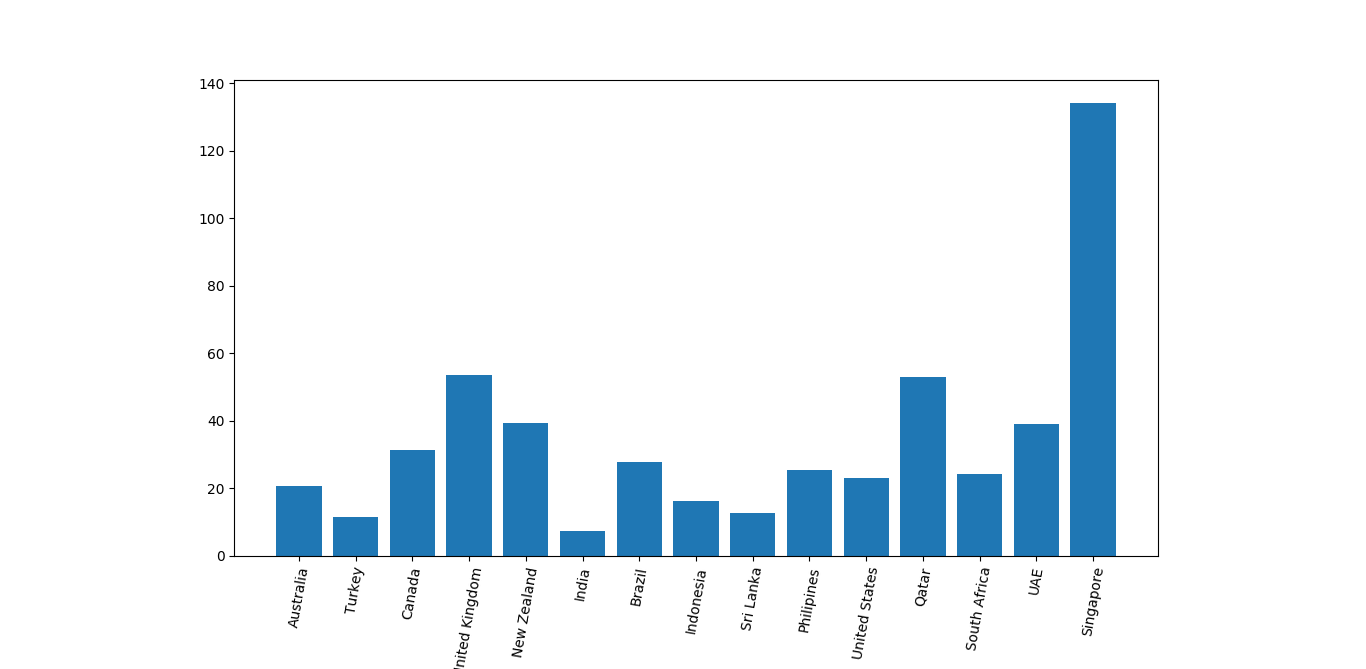
\includegraphics[width=1.2\textwidth]{../images/avgPricePerCountry}
	\caption{Prosecna kolicina novca koja se potrosi u drzavi na restorane}
\end{figure}
\begin{figure}[h!]
	\centering
	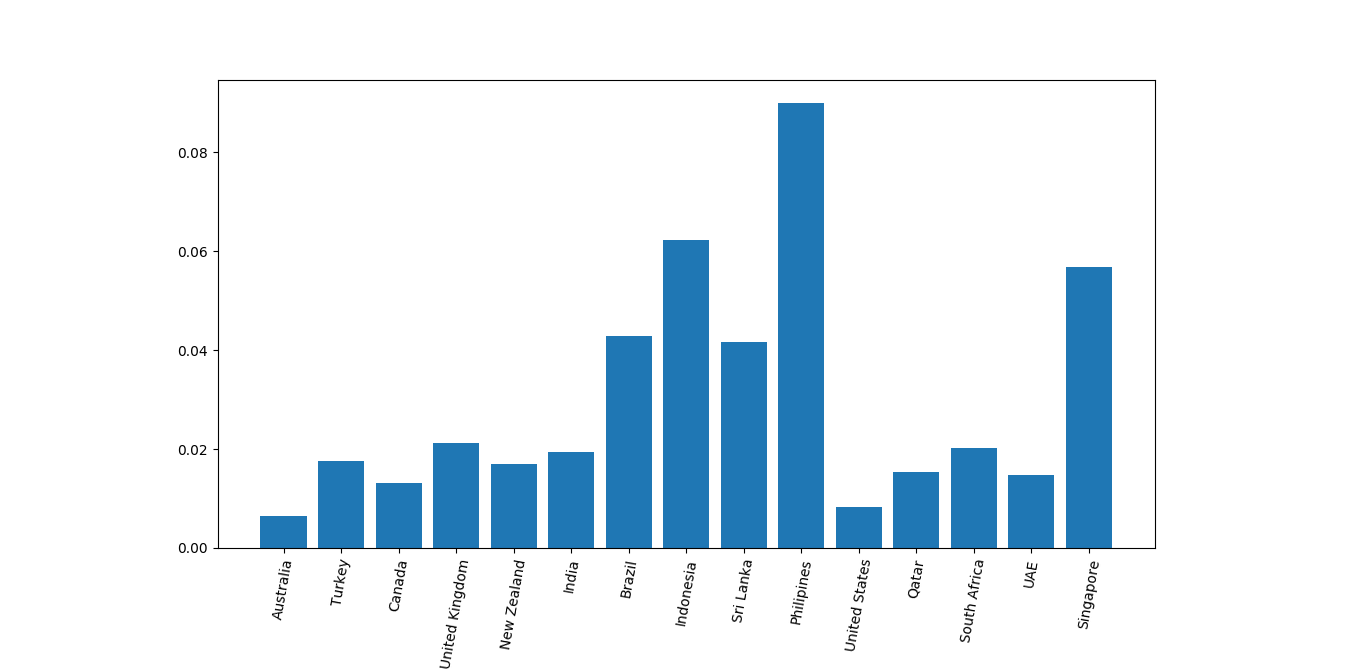
\includegraphics[width=1.2\textwidth]{../images/meanSalaryPercentPerCountry}
	\caption{Uzoracka sredina procenta koji ljudi drzave se potrose na restorane}
\end{figure}
\begin{figure}[h!]
	\centering
	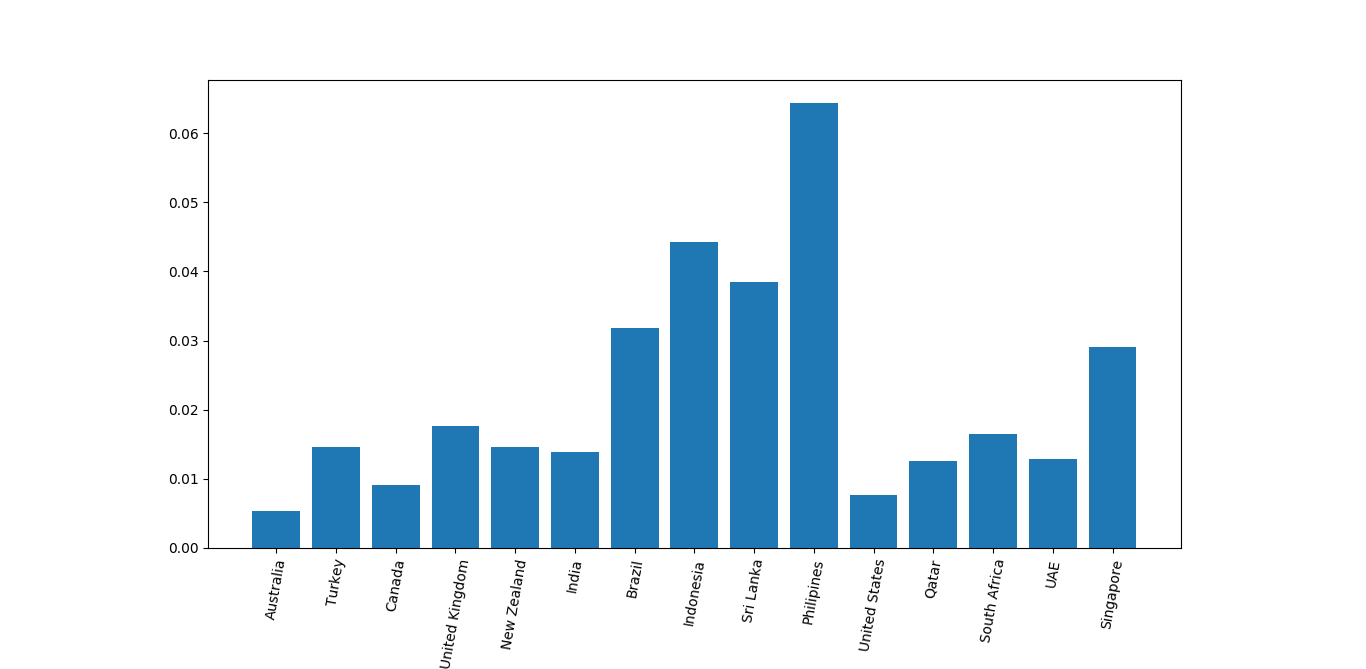
\includegraphics[width=1.2\textwidth]{../images/medianSalaryPercentPerCountry}
	\caption{Medijana procenta koji ljudi drzave se potrose na restorane}
\end{figure}
Primeti se da u drzavama gde su plate vece se potrosi i vise para na restorane (jer je tamo skuplje). S druge strane kada gledamo koliko se procentualno trosi 
Filipini i Indonezija ubedljivo trose najvise u odnosu na svoje plate, ali i Singapur, koji inace trosi najvise para na restorane, je na trecem mestu u trosenju
para u odnosu na platu. Mada kada pogledamo trecu sliku Singapur vise nije na trecem mestu, razlog za to je to sto od svih restorana u pocetnoj tabeli najskuplji 
su u Singapuru, ali nisu svi u Singapuru toliko skupi, iz tog razloga su ih u trecoj tabeli i Sri Lanka i Brazil prestigli.
\newpage

\subsubsection{Frekvencija kuhinja u restoranima}
U svakom restoranu sluze razlicite kuhinje (kineska, italijanska, severnoindijska...). Sada cemo analizirati koja je koliko cesta. Naredni skript ce izgenerisati 
histogram kuhinja i njihovih frekvencija.
\begin{lstlisting}
import pandas as pd
import matplotlib.pyplot as plt

df = pd.read_csv("../data/ComparedPriceAndAvgSalary.csv")

allCuisines = {}
for i, row in df.iterrows():
    cuisines = row["Cuisines"]
    for cuisine in cuisines.replace(" ", "").split(","):
        if cuisine not in allCuisines:
            allCuisines[cuisine] = 1
        else:
            allCuisines[cuisine] += 1

forDeletion = []
others = 0
for k, v in allCuisines.items():
    if v <= 40:
        forDeletion.append(k)
        others += v

for e in forDeletion:
    del allCuisines[e]

allCuisines["Others"] = others

x = range(len(list(allCuisines.keys())))
plt.xticks(x,  list(allCuisines.keys()))
locs, labels = plt.xticks()
plt.setp(labels, rotation=80)
plt.bar(x, list(allCuisines.values()))
plt.show()
plt.close()
\end{lstlisting}
\newpage
Histogram koji ovaj skript generise:
\begin{figure}[h!]
	\centering
	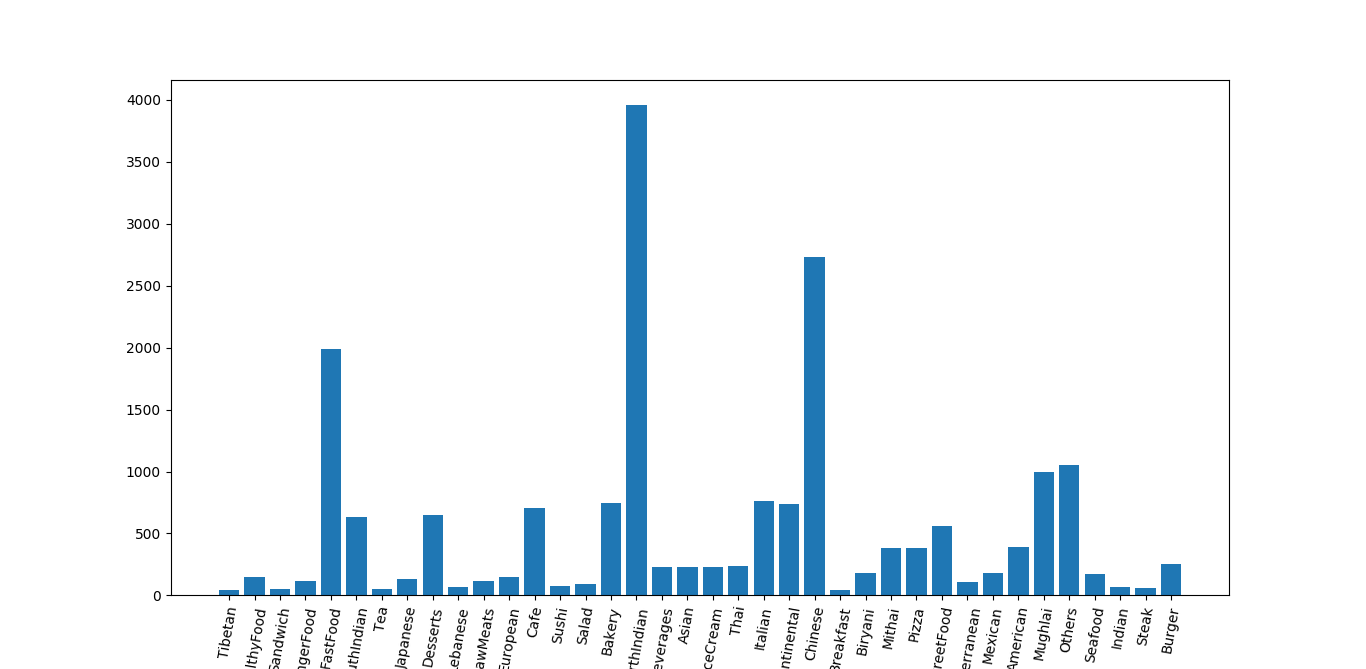
\includegraphics[width=1.2\textwidth]{../images/cuisineHistogram}
	\caption{Histogram kuhinja sa njihovim frekvencijama}
\end{figure}
\newline
Kuhinje kojih ima manje u manje od 40 restorana smo stavili u kolonu Others, jer je 50 malo u odnosu na velicinu tabele (oko 9.5 hiljada), a i zato sto je mnogo 
preglednije ovako. 
Logicno je da severnoindijske kuhinje ima najvise, jer u Indiji ima 8.5 od 9.5 hiljada restorana, slicno vazi i za kinesku kuhinju.

\newpage
\section{Pravila pridruzivanja}
Ovde cemo analizirati koji su cesti skupovi podataka, koji cesto dolaze u paru, koji dolaze ako dodje neki drugi i sa kojom sigurnoscu.
Naredni kod ce izgenerisati ceste skupove i pravila pridruzivanja, posebno smo izdvojili kuhinje i kategoricke ocene i sada cemo proveriti 
koliko cesto idu zajedno i npr. da li je cesta pojava da kineska hrana bude u restoranima koji su ocenjeni dobro i imaju jos i severnoindijsku kuhinju.

\begin{lstlisting}
import pandas as pd
from mlxtend.frequent_patterns import apriori
from mlxtend.frequent_patterns import association_rules

df = pd.read_csv("../data/restaurantsConvertedToEuro.csv")

allCuisines = []
for i, row in df.iterrows():
    cuisines = row["Cuisines"].replace(" ", "").split(",")
    for cuisine in cuisines:
        cuisine = cuisine
        if cuisine not in allCuisines:
            allCuisines.append(cuisine)

allCuisinesData = []
for i in range(len(allCuisines)):
    allCuisinesData.append([])

for i, row in df.iterrows():
    cuisines = row["Cuisines"].replace(" ", "").split(",")
    for ind in range(len(allCuisines)):
        if allCuisines[ind] in cuisines:
            allCuisinesData[ind].append(1)
        else:
            allCuisinesData[ind].append(0)


df2 = pd.DataFrame()
for ind in range(len(allCuisines)):
    df2[allCuisines[ind]] = pd.Series(allCuisinesData[ind], index = df.index)

allRatingTexts = ["Average", "Not rated", "Good", "Very Good", "Excellent", "Poor"]
ratingsData = [[] for i in range(len(allRatingTexts))]

for i, row in df.iterrows():
    for rating in allRatingTexts:
        if rating == row["Rating text"]:
            ratingsData[allRatingTexts.index(rating)].append(1)
        else:
            ratingsData[allRatingTexts.index(rating)].append(0)

for i in range(len(ratingsData)):
    df2[allRatingTexts[i]] = pd.Series(ratingsData[i], index = df2.index)

    
frequent_itemsets = apriori(df2, min_support=0.02, use_colnames=True)
print(frequent_itemsets)
rules = association_rules(frequent_itemsets, metric="confidence", min_threshold=0.3)
print(rules)
\end{lstlisting}
Rezultat izvrsavanja ovog skripta:
\begin{lstlisting}
     support                                  itemsets
0   0.068434                                (Desserts)
1   0.024418                                   (Asian)
2   0.286418                                 (Chinese)
3   0.040872                                (American)
4   0.023685                                (IceCream)
5   0.073674                                    (Cafe)
6   0.080067                                 (Italian)
7   0.039929                                   (Pizza)
8   0.077971                                  (Bakery)
9   0.208132                                (FastFood)
10  0.026305                                  (Burger)
11  0.023894                               (Beverages)
12  0.024523                                    (Thai)
13  0.077133                             (Continental)
14  0.415007                             (NorthIndian)
15  0.104171                                 (Mughlai)
16  0.066653                             (SouthIndian)
17  0.058898                              (StreetFood)
18  0.039824                                  (Mithai)
19  0.391323                                 (Average)
20  0.225110                               (Not rated)
21  0.219660                                    (Good)
22  0.112974                               (Very Good)
23  0.031440                               (Excellent)
24  0.029868                        (Desserts, Bakery)
25  0.023370                       (Desserts, Average)
26  0.021065                          (Desserts, Good)
27  0.023056                        (Chinese, Italian)
28  0.048837                       (FastFood, Chinese)
29  0.031754                    (Continental, Chinese)
..       ...                                       ...
50  0.043492                          (FastFood, Good)
51  0.049046                (Continental, NorthIndian)
52  0.020226                    (Continental, Average)
53  0.029449                       (Continental, Good)
54  0.020122                  (Continental, Very Good)
55  0.087089                    (Mughlai, NorthIndian)
56  0.042444                (SouthIndian, NorthIndian)
57  0.193356                    (Average, NorthIndian)
58  0.098826                  (Not rated, NorthIndian)
59  0.078914                       (Good, NorthIndian)
60  0.028925                  (Very Good, NorthIndian)
61  0.051981                        (Average, Mughlai)
62  0.020960                      (Not rated, Mughlai)
63  0.020541                           (Good, Mughlai)
64  0.033326                    (Average, SouthIndian)
65  0.025676                      (Mithai, StreetFood)
66  0.025781                     (Average, StreetFood)
67  0.024733          (FastFood, Chinese, NorthIndian)
68  0.027562              (FastFood, Average, Chinese)
69  0.026514       (Continental, Chinese, NorthIndian)
70  0.038252           (Mughlai, Chinese, NorthIndian)
71  0.029030       (SouthIndian, Chinese, NorthIndian)
72  0.098407           (Average, Chinese, NorthIndian)
73  0.031754         (Not rated, Chinese, NorthIndian)
74  0.036575              (Good, Chinese, NorthIndian)
75  0.023475               (Average, Mughlai, Chinese)
76  0.031021          (FastFood, Average, NorthIndian)
77  0.046426           (Average, Mughlai, NorthIndian)
78  0.021798       (Average, SouthIndian, NorthIndian)
79  0.022742  (Average, Mughlai, Chinese, NorthIndian)

[80 rows x 2 columns]
                        antecedents             consequents  antecedent support  consequent support   support  confidence       lift  leverage  conviction
0                        (Desserts)               (Average)            0.068434            0.391323  0.023370    0.341501   0.872684 -0.003410    0.924340
1                         (Average)               (Chinese)            0.391323            0.286418  0.139698    0.356990   1.246395  0.027616    1.109752
2                         (Chinese)               (Average)            0.286418            0.391323  0.139698    0.487742   1.246395  0.027616    1.188225
3                          (Mithai)            (StreetFood)            0.039824            0.058898  0.025676    0.644737  10.946760  0.023330    2.649029
4                      (StreetFood)                (Mithai)            0.058898            0.039824  0.025676    0.435943  10.946760  0.023330    1.702268
5                       (Not rated)           (NorthIndian)            0.225110            0.415007  0.098826    0.439013   1.057844  0.005404    1.042792
6                         (Mughlai)               (Chinese)            0.104171            0.286418  0.039719    0.381288   1.331228  0.009883    1.153334
7                     (Continental)               (Chinese)            0.077133            0.286418  0.031754    0.411685   1.437357  0.009662    1.212925
8            (Continental, Chinese)           (NorthIndian)            0.031754            0.415007  0.026514    0.834983   2.011973  0.013336    3.545056
9        (Continental, NorthIndian)               (Chinese)            0.049046            0.286418  0.026514    0.540598   1.887446  0.012467    1.553286
10                    (Continental)  (Chinese, NorthIndian)            0.077133            0.186753  0.026514    0.343750   1.840664  0.012110    1.239233
11                        (Mughlai)           (NorthIndian)            0.104171            0.415007  0.087089    0.836016   2.014461  0.043857    3.567379
12           (Average, SouthIndian)           (NorthIndian)            0.033326            0.415007  0.021798    0.654088   1.576088  0.007968    1.691161
13       (SouthIndian, NorthIndian)               (Average)            0.042444            0.391323  0.021798    0.513580   1.312422  0.005189    1.251342
14                    (SouthIndian)  (Average, NorthIndian)            0.066653            0.193356  0.021798    0.327044   1.691411  0.008911    1.198658
15                        (Italian)                  (Good)            0.080067            0.219660  0.029973    0.374346   1.704201  0.012385    1.247237
16                    (SouthIndian)               (Average)            0.066653            0.391323  0.033326    0.500000   1.277718  0.007244    1.217355
17                        (Average)           (NorthIndian)            0.391323            0.415007  0.193356    0.494108   1.190601  0.030954    1.156359
18                    (NorthIndian)               (Average)            0.415007            0.391323  0.193356    0.465909   1.190601  0.030954    1.139651
19                        (Mughlai)               (Average)            0.104171            0.391323  0.051981    0.498994   1.275147  0.011216    1.214910
20                    (Continental)               (Italian)            0.077133            0.080067  0.028715    0.372283   4.649634  0.022539    1.465521
21                        (Italian)           (Continental)            0.080067            0.077133  0.028715    0.358639   4.649634  0.022539    1.438920
22                          (Pizza)              (FastFood)            0.039929            0.208132  0.020436    0.511811   2.459064  0.012126    1.622051
23           (SouthIndian, Chinese)           (NorthIndian)            0.036051            0.415007  0.029030    0.805233   1.940285  0.014068    3.003544
24       (SouthIndian, NorthIndian)               (Chinese)            0.042444            0.286418  0.029030    0.683951   2.387946  0.016873    2.257818
25                    (SouthIndian)  (Chinese, NorthIndian)            0.066653            0.186753  0.029030    0.435535   2.332139  0.016582    1.440738
26                    (SouthIndian)               (Chinese)            0.066653            0.286418  0.036051    0.540881   1.888431  0.016961    1.554240
27                    (Continental)                  (Good)            0.077133            0.219660  0.029449    0.381793   1.738108  0.012506    1.262264
28               (Average, Mughlai)               (Chinese)            0.051981            0.286418  0.023475    0.451613   1.576762  0.008587    1.301238
29               (Mughlai, Chinese)               (Average)            0.039719            0.391323  0.023475    0.591029   1.510337  0.007932    1.488314
..                              ...                     ...                 ...                 ...       ...         ...        ...       ...         ...
37      (Average, Mughlai, Chinese)           (NorthIndian)            0.023475            0.415007  0.022742    0.968750   2.334296  0.012999   18.719765
38  (Average, Mughlai, NorthIndian)               (Chinese)            0.046426            0.286418  0.022742    0.489842   1.710235  0.009444    1.398747
39  (Mughlai, Chinese, NorthIndian)               (Average)            0.038252            0.391323  0.022742    0.594521   1.519260  0.007773    1.501130
40               (Average, Mughlai)  (Chinese, NorthIndian)            0.051981            0.186753  0.022742    0.437500   2.342663  0.013034    1.445772
41               (Mughlai, Chinese)  (Average, NorthIndian)            0.039719            0.193356  0.022742    0.572559   2.961172  0.015062    1.887149
42                           (Cafe)                  (Good)            0.073674            0.219660  0.023894    0.324324   1.476480  0.007711    1.154903
43                       (Desserts)                (Bakery)            0.068434            0.077971  0.029868    0.436447   5.597552  0.024532    1.636100
44                         (Bakery)              (Desserts)            0.077971            0.068434  0.029868    0.383065   5.597552  0.024532    1.509989
45                         (Bakery)              (FastFood)            0.077971            0.208132  0.023580    0.302419   1.453014  0.007352    1.135163
46                       (FastFood)               (Average)            0.208132            0.391323  0.103437    0.496979   1.269998  0.021991    1.210043
47              (FastFood, Chinese)           (NorthIndian)            0.048837            0.415007  0.024733    0.506438   1.220310  0.004465    1.185246
48          (FastFood, NorthIndian)               (Chinese)            0.050828            0.286418  0.024733    0.486598   1.698909  0.010175    1.389909
49               (Average, Chinese)           (NorthIndian)            0.139698            0.415007  0.098407    0.704426   1.697382  0.040431    1.979176
50           (Average, NorthIndian)               (Chinese)            0.193356            0.286418  0.098407    0.508943   1.776925  0.043027    1.453156
51           (Chinese, NorthIndian)               (Average)            0.186753            0.391323  0.098407    0.526936   1.346552  0.025326    1.286670
52                        (Chinese)  (Average, NorthIndian)            0.286418            0.193356  0.098407    0.343578   1.776925  0.043027    1.228851
53               (Mughlai, Chinese)           (NorthIndian)            0.039719            0.415007  0.038252    0.963061   2.320587  0.021768   15.836587
54           (Mughlai, NorthIndian)               (Chinese)            0.087089            0.286418  0.038252    0.439230   1.533528  0.013308    1.272504
55                        (Mughlai)  (Chinese, NorthIndian)            0.104171            0.186753  0.038252    0.367203   1.966248  0.018798    1.285163
56              (FastFood, Chinese)               (Average)            0.048837            0.391323  0.027562    0.564378   1.442231  0.008451    1.397260
57                         (Bakery)               (Average)            0.077971            0.391323  0.031650    0.405914   1.037287  0.001138    1.024561
58             (Not rated, Chinese)           (NorthIndian)            0.057745            0.415007  0.031754    0.549909   1.325059  0.007790    1.299722
59         (Not rated, NorthIndian)               (Chinese)            0.098826            0.286418  0.031754    0.321315   1.121839  0.003449    1.051419
60               (Average, Mughlai)           (NorthIndian)            0.051981            0.415007  0.046426    0.893145   2.152119  0.024854    5.474648
61           (Mughlai, NorthIndian)               (Average)            0.087089            0.391323  0.046426    0.533093   1.362284  0.012347    1.303636
62                        (Mughlai)  (Average, NorthIndian)            0.104171            0.193356  0.046426    0.445674   2.304944  0.026284    1.455180
63                    (SouthIndian)           (NorthIndian)            0.066653            0.415007  0.042444    0.636792   1.534413  0.014783    1.610629
64                  (Good, Chinese)           (NorthIndian)            0.057640            0.415007  0.036575    0.634545   1.528998  0.012654    1.600726
65              (Good, NorthIndian)               (Chinese)            0.078914            0.286418  0.036575    0.463479   1.618193  0.013973    1.330018
66                        (Italian)           (NorthIndian)            0.080067            0.415007  0.030916    0.386126   0.930407 -0.002312    0.952952

[67 rows x 9 columns]
                        antecedents             consequents  antecedent support  consequent support   support  confidence       lift  leverage  conviction
1                         (Average)               (Chinese)            0.391323            0.286418  0.139698    0.356990   1.246395  0.027616    1.109752
2                         (Chinese)               (Average)            0.286418            0.391323  0.139698    0.487742   1.246395  0.027616    1.188225
3                          (Mithai)            (StreetFood)            0.039824            0.058898  0.025676    0.644737  10.946760  0.023330    2.649029
4                      (StreetFood)                (Mithai)            0.058898            0.039824  0.025676    0.435943  10.946760  0.023330    1.702268
5                       (Not rated)           (NorthIndian)            0.225110            0.415007  0.098826    0.439013   1.057844  0.005404    1.042792
6                         (Mughlai)               (Chinese)            0.104171            0.286418  0.039719    0.381288   1.331228  0.009883    1.153334
7                     (Continental)               (Chinese)            0.077133            0.286418  0.031754    0.411685   1.437357  0.009662    1.212925
8            (Continental, Chinese)           (NorthIndian)            0.031754            0.415007  0.026514    0.834983   2.011973  0.013336    3.545056
9        (Continental, NorthIndian)               (Chinese)            0.049046            0.286418  0.026514    0.540598   1.887446  0.012467    1.553286
10                    (Continental)  (Chinese, NorthIndian)            0.077133            0.186753  0.026514    0.343750   1.840664  0.012110    1.239233
11                        (Mughlai)           (NorthIndian)            0.104171            0.415007  0.087089    0.836016   2.014461  0.043857    3.567379
12           (Average, SouthIndian)           (NorthIndian)            0.033326            0.415007  0.021798    0.654088   1.576088  0.007968    1.691161
13       (SouthIndian, NorthIndian)               (Average)            0.042444            0.391323  0.021798    0.513580   1.312422  0.005189    1.251342
14                    (SouthIndian)  (Average, NorthIndian)            0.066653            0.193356  0.021798    0.327044   1.691411  0.008911    1.198658
15                        (Italian)                  (Good)            0.080067            0.219660  0.029973    0.374346   1.704201  0.012385    1.247237
16                    (SouthIndian)               (Average)            0.066653            0.391323  0.033326    0.500000   1.277718  0.007244    1.217355
17                        (Average)           (NorthIndian)            0.391323            0.415007  0.193356    0.494108   1.190601  0.030954    1.156359
18                    (NorthIndian)               (Average)            0.415007            0.391323  0.193356    0.465909   1.190601  0.030954    1.139651
19                        (Mughlai)               (Average)            0.104171            0.391323  0.051981    0.498994   1.275147  0.011216    1.214910
20                    (Continental)               (Italian)            0.077133            0.080067  0.028715    0.372283   4.649634  0.022539    1.465521
21                        (Italian)           (Continental)            0.080067            0.077133  0.028715    0.358639   4.649634  0.022539    1.438920
22                          (Pizza)              (FastFood)            0.039929            0.208132  0.020436    0.511811   2.459064  0.012126    1.622051
23           (SouthIndian, Chinese)           (NorthIndian)            0.036051            0.415007  0.029030    0.805233   1.940285  0.014068    3.003544
24       (SouthIndian, NorthIndian)               (Chinese)            0.042444            0.286418  0.029030    0.683951   2.387946  0.016873    2.257818
25                    (SouthIndian)  (Chinese, NorthIndian)            0.066653            0.186753  0.029030    0.435535   2.332139  0.016582    1.440738
26                    (SouthIndian)               (Chinese)            0.066653            0.286418  0.036051    0.540881   1.888431  0.016961    1.554240
27                    (Continental)                  (Good)            0.077133            0.219660  0.029449    0.381793   1.738108  0.012506    1.262264
28               (Average, Mughlai)               (Chinese)            0.051981            0.286418  0.023475    0.451613   1.576762  0.008587    1.301238
29               (Mughlai, Chinese)               (Average)            0.039719            0.391323  0.023475    0.591029   1.510337  0.007932    1.488314
30                       (Desserts)                  (Good)            0.068434            0.219660  0.021065    0.307810   1.401300  0.006032    1.127349
..                              ...                     ...                 ...                 ...       ...         ...        ...       ...         ...
35          (FastFood, NorthIndian)               (Average)            0.050828            0.391323  0.031021    0.610309   1.559607  0.011131    1.561950
37      (Average, Mughlai, Chinese)           (NorthIndian)            0.023475            0.415007  0.022742    0.968750   2.334296  0.012999   18.719765
38  (Average, Mughlai, NorthIndian)               (Chinese)            0.046426            0.286418  0.022742    0.489842   1.710235  0.009444    1.398747
39  (Mughlai, Chinese, NorthIndian)               (Average)            0.038252            0.391323  0.022742    0.594521   1.519260  0.007773    1.501130
40               (Average, Mughlai)  (Chinese, NorthIndian)            0.051981            0.186753  0.022742    0.437500   2.342663  0.013034    1.445772
41               (Mughlai, Chinese)  (Average, NorthIndian)            0.039719            0.193356  0.022742    0.572559   2.961172  0.015062    1.887149
42                           (Cafe)                  (Good)            0.073674            0.219660  0.023894    0.324324   1.476480  0.007711    1.154903
43                       (Desserts)                (Bakery)            0.068434            0.077971  0.029868    0.436447   5.597552  0.024532    1.636100
44                         (Bakery)              (Desserts)            0.077971            0.068434  0.029868    0.383065   5.597552  0.024532    1.509989
45                         (Bakery)              (FastFood)            0.077971            0.208132  0.023580    0.302419   1.453014  0.007352    1.135163
46                       (FastFood)               (Average)            0.208132            0.391323  0.103437    0.496979   1.269998  0.021991    1.210043
47              (FastFood, Chinese)           (NorthIndian)            0.048837            0.415007  0.024733    0.506438   1.220310  0.004465    1.185246
48          (FastFood, NorthIndian)               (Chinese)            0.050828            0.286418  0.024733    0.486598   1.698909  0.010175    1.389909
49               (Average, Chinese)           (NorthIndian)            0.139698            0.415007  0.098407    0.704426   1.697382  0.040431    1.979176
50           (Average, NorthIndian)               (Chinese)            0.193356            0.286418  0.098407    0.508943   1.776925  0.043027    1.453156
51           (Chinese, NorthIndian)               (Average)            0.186753            0.391323  0.098407    0.526936   1.346552  0.025326    1.286670
52                        (Chinese)  (Average, NorthIndian)            0.286418            0.193356  0.098407    0.343578   1.776925  0.043027    1.228851
53               (Mughlai, Chinese)           (NorthIndian)            0.039719            0.415007  0.038252    0.963061   2.320587  0.021768   15.836587
54           (Mughlai, NorthIndian)               (Chinese)            0.087089            0.286418  0.038252    0.439230   1.533528  0.013308    1.272504
55                        (Mughlai)  (Chinese, NorthIndian)            0.104171            0.186753  0.038252    0.367203   1.966248  0.018798    1.285163
56              (FastFood, Chinese)               (Average)            0.048837            0.391323  0.027562    0.564378   1.442231  0.008451    1.397260
57                         (Bakery)               (Average)            0.077971            0.391323  0.031650    0.405914   1.037287  0.001138    1.024561
58             (Not rated, Chinese)           (NorthIndian)            0.057745            0.415007  0.031754    0.549909   1.325059  0.007790    1.299722
59         (Not rated, NorthIndian)               (Chinese)            0.098826            0.286418  0.031754    0.321315   1.121839  0.003449    1.051419
60               (Average, Mughlai)           (NorthIndian)            0.051981            0.415007  0.046426    0.893145   2.152119  0.024854    5.474648
61           (Mughlai, NorthIndian)               (Average)            0.087089            0.391323  0.046426    0.533093   1.362284  0.012347    1.303636
62                        (Mughlai)  (Average, NorthIndian)            0.104171            0.193356  0.046426    0.445674   2.304944  0.026284    1.455180
63                    (SouthIndian)           (NorthIndian)            0.066653            0.415007  0.042444    0.636792   1.534413  0.014783    1.610629
64                  (Good, Chinese)           (NorthIndian)            0.057640            0.415007  0.036575    0.634545   1.528998  0.012654    1.600726
65              (Good, NorthIndian)               (Chinese)            0.078914            0.286418  0.036575    0.463479   1.618193  0.013973    1.330018

[64 rows x 9 columns]
\end{lstlisting}
Prvo smo ispisali sve ceste skupove i njihove podrske, odabrali smo da minimalna podrska bude 0.02, jer se tako dobijaju najbolja pravila, a i ostale mere u 
kasnijem radu su ispale najbolje. Zatim smo od pravila asocijacije uzeli ona koja imaju lift veci od 1.

\newpage
\section{Klasifikacija}
U ovom delu cemo na osnovu podataka koje imamo i njihovih vrednosti odredjenih atributa predvidjati koju vrednost klasnog atributa bi imala neka nova instanca.
Za to cemo koristiti algoritme za klasifikaciju kao sto su SVM (Support Vector Machine), Decision Tree i Naive Bayes, takodje 
cemo koristi neuronske mreze i posle proverati ko daje najvecu preciznost pri predvidjanju.
\newline
Radicemo 4 razlicite klasifikacije. To su predvidjanje drzave, predvidjanje kategoricke cene, kategoricke ocene i kategorickog broja glasova. Za sve se koriste 
razlicti atributi koji ni na koji direktan nacin nisu povezani sa klasnim atributom (ako se predvidja drzava, bilo kakva informacija o lokaciji restorana nece 
biti poznata...).

\subsection{Drzava: kuhinje, prikupljena ocena, prosecna cena u evrima, broj glasova}
Na osnovu ovih atributa ce se predvidjati koja je drzava u pitanju.
Atributi kuhinje predstavljaju sve kuhinje koje se pojavljuju u nasim podacima, to su binarni atributi koji se generisu sledecim skriptom:

\begin{lstlisting}
import pandas as pd

df = pd.read_csv("ComparedPriceAndAvgSalary.csv")

allCuisines = []
for i, row in df.iterrows():
    cuisines = row["Cuisines"]
    for cuisine in cuisines.replace(" ", "").split(","):
        if cuisine not in allCuisines:
            allCuisines.append(cuisine)
            
allCuisinesData = [[] for i in range(len(allCuisines))]

for i, row in df.iterrows():
    for k in range(len(allCuisines)):
        if allCuisines[k] in row["Cuisines"].replace(" ", "").split(","):
            allCuisinesData[k].append(1)
        else:
            allCuisinesData[k].append(0)
            
for cuisineData in allCuisinesData:
    df[allCuisinesData.index(cuisineData)] = pd.Series(cuisineData, index = df.index)
    
with open("AddedCuisineCols.csv", "w") as csvFile:
    csv = df.to_csv()
    csvFile.write(csv)

\end{lstlisting}


\begin{figure}[h!]
	\centering
	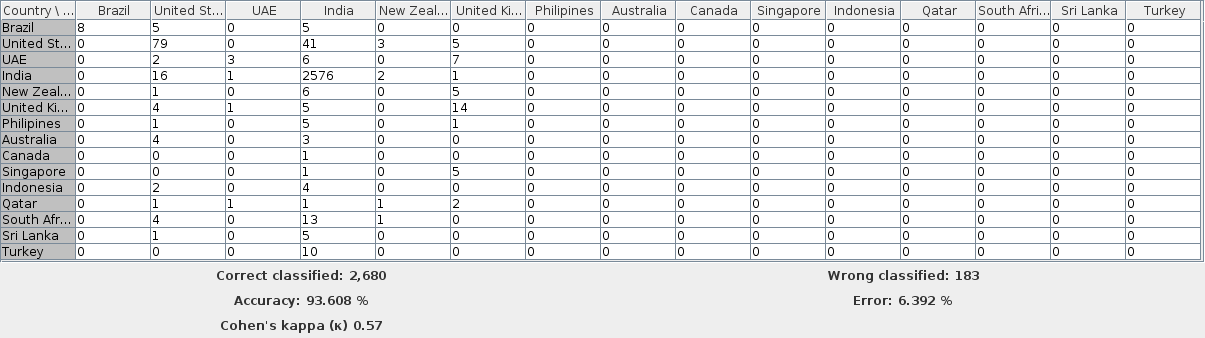
\includegraphics[width=1.1\textwidth]{countryClassificationTest/DecisionTree}
	\caption{Matrica konfuzije za test skup za klasifikaciju sa klasifikatorom Decision Tree}
\end{figure}
\begin{figure}[h!]
	\centering
	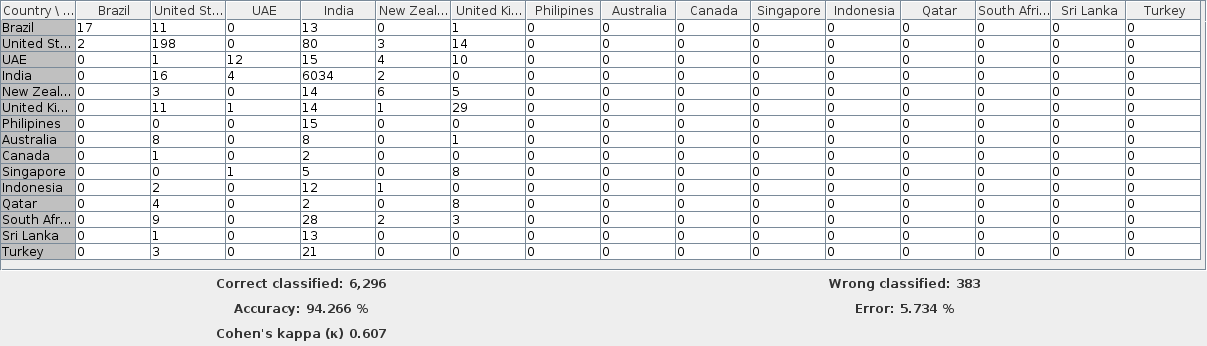
\includegraphics[width=1.1\textwidth]{countryClassificationTraining/DecisionTree}
	\caption{Matrica konfuzije za trening skup za klasifikaciju sa klasifikatorom Decision Tree}
\end{figure}
\newline
\begin{figure}[h!]
	\centering
	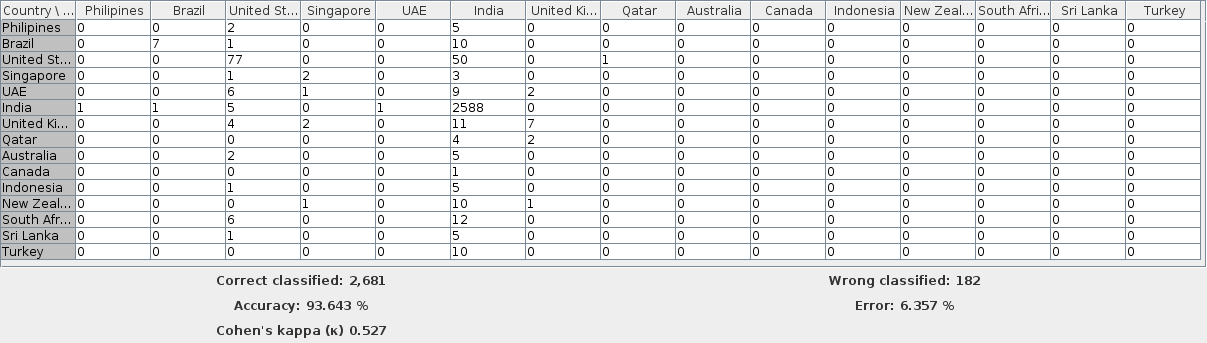
\includegraphics[width=1.1\textwidth]{countryClassificationTest/SVM}
	\caption{Matrica konfuzije za test skup za klasifikaciju sa klasifikatorom SVM}
\end{figure}
\begin{figure}[h!]
	\centering
	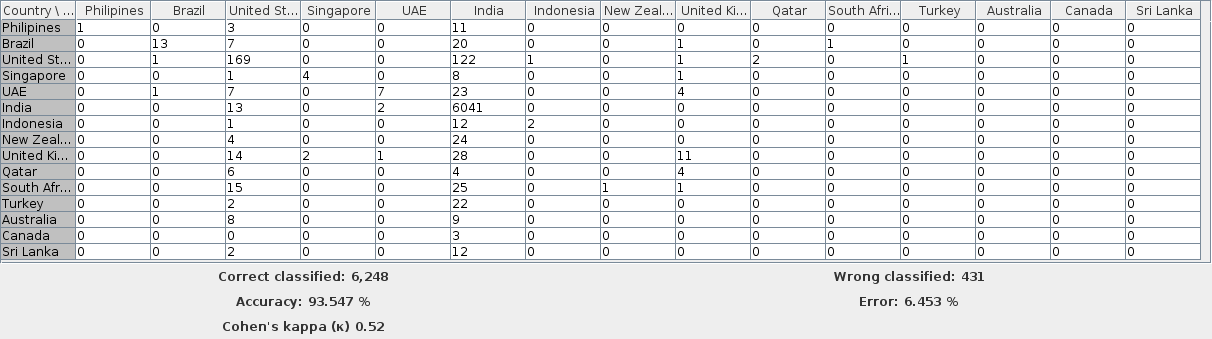
\includegraphics[width=1.1\textwidth]{countryClassificationTraining/SVM}
	\caption{Matrica konfuzije za trening skup za klasifikaciju sa klasifikatorom SVM}
\end{figure}
\newline
\begin{figure}[h!]
	\centering
	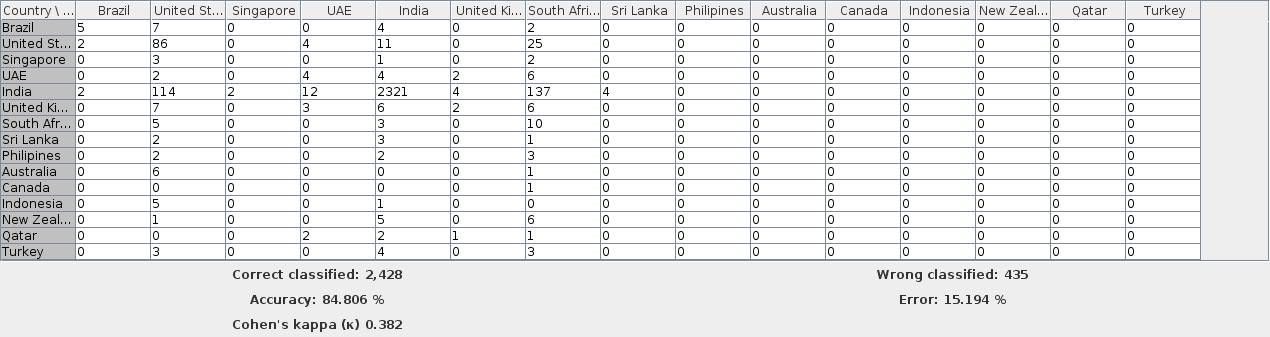
\includegraphics[width=1.1\textwidth]{countryClassificationTest/NaiveBayes}
	\caption{Matrica konfuzije za test skup za klasifikaciju sa klasifikatorom Naive Bayes}
\end{figure}
\begin{figure}[h!]
	\centering
	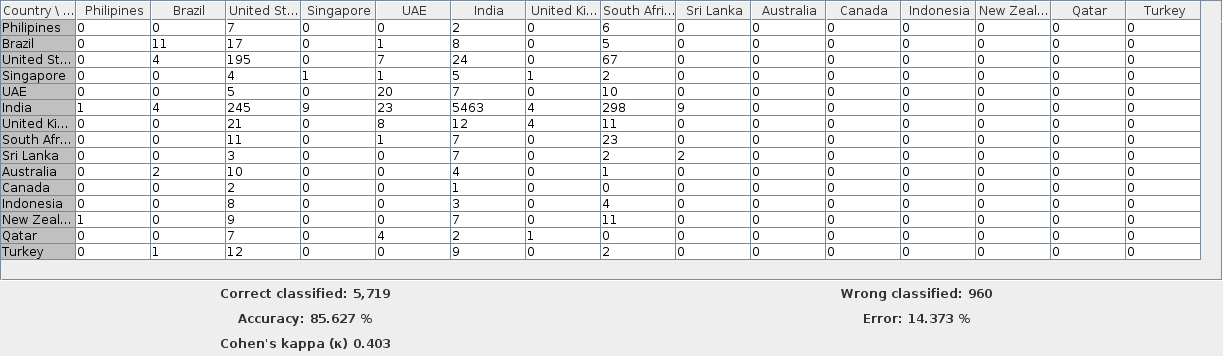
\includegraphics[width=1.1\textwidth]{countryClassificationTraining/NaiveBayes}
	\caption{Matrica konfuzije za trening skup za klasifikaciju sa klasifikatorom Naive Bayes}
\end{figure}
\newline
\begin{figure}[h!]
	\centering
	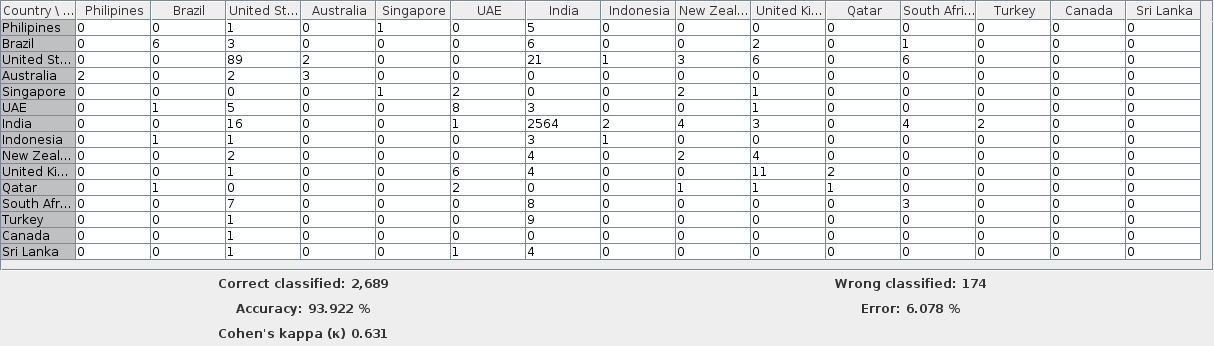
\includegraphics[width=1.1\textwidth]{countryClassificationTest/RProp}
	\caption{Matrica konfuzije za test skup za klasifikaciju sa klasifikatorom RProp MLP}
\end{figure}
\begin{figure}[h!]
	\centering
	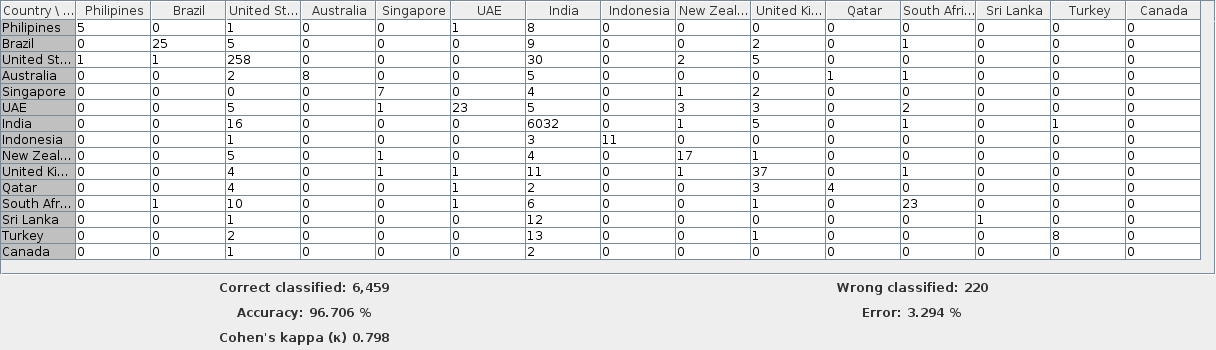
\includegraphics[width=1.1\textwidth]{countryClassificationTraining/RProp}
	\caption{Matrica konfuzije za trening skup za klasifikaciju sa klasifikatorom RProp MLP}
\end{figure}


\newpage
\subsection{Kategoricka ocena: geografska sirina, geografska duzina, raspon cena, prosecna cena u evrima, odnos cene restorana i plate u toj drzavi}
Na osnovu ovih atributa ce se predvidjati koja je kategoricka ocena (Excellent, Very Good, Good...) u pitanju.

\begin{figure}[h!]
	\centering
	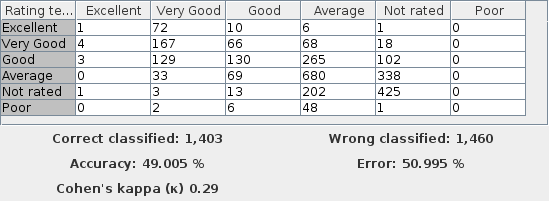
\includegraphics[width=1.1\textwidth]{ratingClassificationTest/DecisionTree}
	\caption{Matrica konfuzije za test skup za klasifikaciju sa klasifikatorom Decision Tree}
\end{figure}
\begin{figure}[h!]
	\centering
	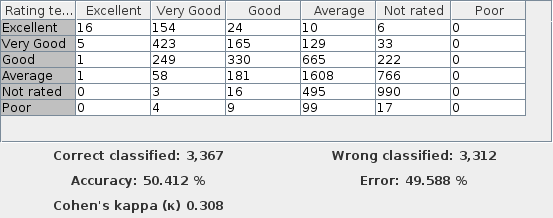
\includegraphics[width=1.1\textwidth]{ratingClassificationTraining/DecisionTree}
	\caption{Matrica konfuzije za trening skup za klasifikaciju sa klasifikatorom Decision Tree}
\end{figure}
\newline
\begin{figure}[h!]
	\centering
	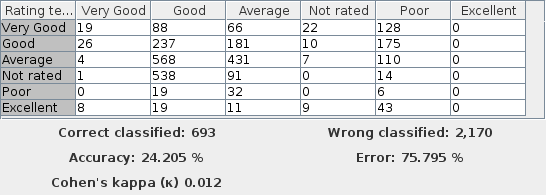
\includegraphics[width=1.1\textwidth]{ratingClassificationTest/SVM}
	\caption{Matrica konfuzije za test skup za klasifikaciju sa klasifikatorom SVM}
\end{figure}
\begin{figure}[h!]
	\centering
	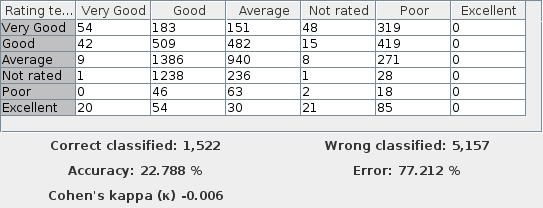
\includegraphics[width=1.1\textwidth]{ratingClassificationTraining/SVM}
	\caption{Matrica konfuzije za trening skup za klasifikaciju sa klasifikatorom SVM}
\end{figure}
\newline
\begin{figure}[h!]
	\centering
	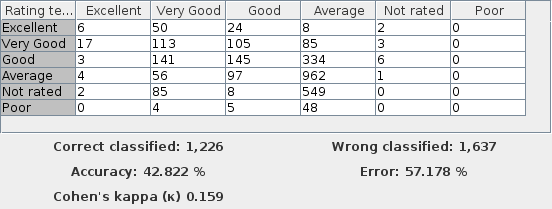
\includegraphics[width=1.1\textwidth]{ratingClassificationTest/NaiveBayes}
	\caption{Matrica konfuzije za test skup za klasifikaciju sa klasifikatorom Naive Bayes}
\end{figure}
\begin{figure}[h!]
	\centering
	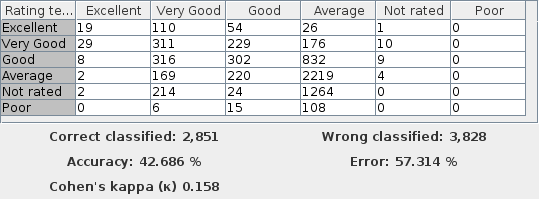
\includegraphics[width=1.1\textwidth]{ratingClassificationTraining/NaiveBayes}
	\caption{Matrica konfuzije za trening skup za klasifikaciju sa klasifikatorom Naive Bayes}
\end{figure}
\newline
\begin{figure}[h!]
	\centering
	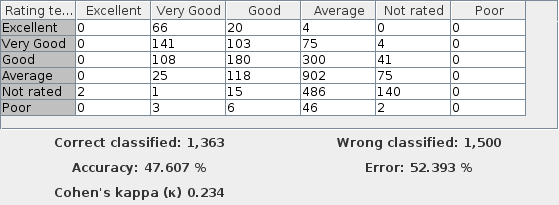
\includegraphics[width=1.1\textwidth]{ratingClassificationTest/RProp}
	\caption{Matrica konfuzije za test skup za klasifikaciju sa klasifikatorom RProp MLP}
\end{figure}
\begin{figure}[h!]
	\centering
	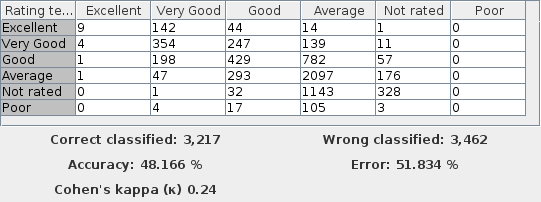
\includegraphics[width=1.1\textwidth]{ratingClassificationTraining/RProp}
	\caption{Matrica konfuzije za trening skup za klasifikaciju sa klasifikatorom RProp MLP}
\end{figure}


\newpage
\subsection{Kategoricki broj glasova: geografska sirina, geografska duzina, raspon cena, prikupljena ocena, prosecna cena u evrima, 
odnos cene restorana i plate u toj drzavi}
Na osnovu ovih atributa ce se predvidjati koji je kategoricki broj glasova (Low, Medium, High) u pitanju. 
\newline 
Podaci koji su korisceni su generisani iz tabele AddedCategoricalVotes.csv koja je izgenerisana sledecim skriptom:


\begin{lstlisting}
import pandas as pd

df = pd.read_csv("../data/ComparedPriceAndAvgSalary.csv")

df = df.sort_values(by = "Votes")

votesData = []
for i, row in df.iterrows():
    if i < len(df.index)/3.0:
        votesData.append("Low")
    elif  i < len(df.index)*2/3.0:
        votesData.append("Medium")
    else:
        votesData.append("High")
        
df["# Votes"] = pd.Series(votesData, index = df.index)

with open("AddedCategoricalVotes.csv", "w") as csvFile:
    csv = df.to_csv()
    csvFile.write(csv)
\end{lstlisting}
Podaci su prvo sortirani neopadajuce po koloni Votes, zatim je prvoj trecini dodata vrednost Low, drugoj trecini Medium, a trecoj High za novi kategoricki 
atribut \# Votes.

\begin{figure}[h!]
	\centering
	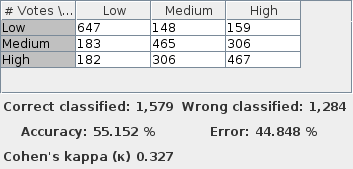
\includegraphics[width=0.85\textwidth]{votesClassificationTest/DecisionTree}
	\caption{Matrica konfuzije za test skup za klasifikaciju sa klasifikatorom Decision Tree}
\end{figure}
\begin{figure}[h!]
	\centering
	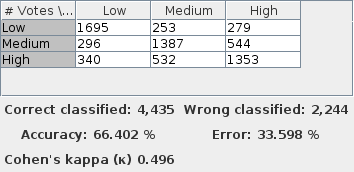
\includegraphics[width=0.85\textwidth]{votesClassificationTraining/DecisionTree}
	\caption{Matrica konfuzije za trening skup za klasifikaciju sa klasifikatorom Decision Tree}
\end{figure}
\newline
\begin{figure}[h!]
	\centering
	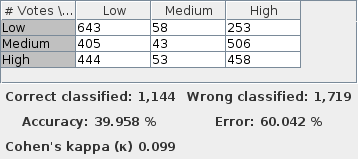
\includegraphics[width=0.85\textwidth]{votesClassificationTest/SVM}
	\caption{Matrica konfuzije za test skup za klasifikaciju sa klasifikatorom SVM}
\end{figure}
\begin{figure}[h!]
	\centering
	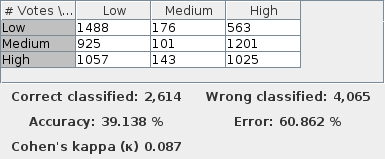
\includegraphics[width=0.85\textwidth]{votesClassificationTraining/SVM}
	\caption{Matrica konfuzije za trening skup za klasifikaciju sa klasifikatorom SVM}
\end{figure}
\newline
\begin{figure}[h!]
	\centering
	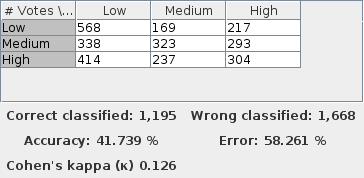
\includegraphics[width=0.85\textwidth]{votesClassificationTest/NaiveBayes}
	\caption{Matrica konfuzije za test skup za klasifikaciju sa klasifikatorom Naive Bayes}
\end{figure}
\begin{figure}[h!]
	\centering
	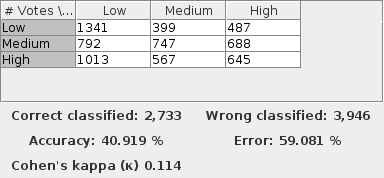
\includegraphics[width=0.85\textwidth]{votesClassificationTraining/NaiveBayes}
	\caption{Matrica konfuzije za trening skup za klasifikaciju sa klasifikatorom Naive Bayes}
\end{figure}
\newline
\begin{figure}[h!]
	\centering
	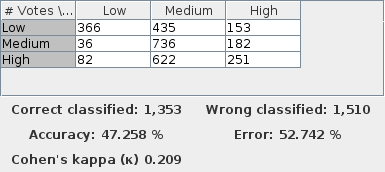
\includegraphics[width=0.85\textwidth]{votesClassificationTest/RProp}
	\caption{Matrica konfuzije za test skup za klasifikaciju sa klasifikatorom RProp MLP}
\end{figure}
\begin{figure}[h!]
	\centering
	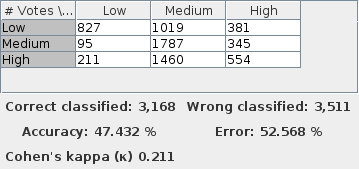
\includegraphics[width=0.85\textwidth]{votesClassificationTraining/RProp}
	\caption{Matrica konfuzije za trening skup za klasifikaciju sa klasifikatorom RProp MLP}
\end{figure}

\newpage
\subsection{Kategoricka cena: prikupljena ocena, broj glasova, kuhinje}
Na osnovu ovih atributa ce se predvidjati koja je kategoricka cena (Very Low, Low, High, Very High) u pitanju.
Kategoricka cena se podacima dodeljuje tako sto se posmatra vrednost kolone odnos cene u restoranu i prosecne plate u drzavi i to se deli na intervale (od 0\% do 
1\%, od 1\% do 2\%, od 2\% do 4.5\% i od 4.5\% do 100\%).

\begin{figure}[h!]
	\centering
	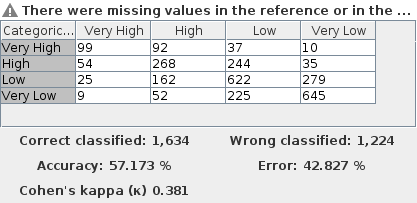
\includegraphics[width=1.1\textwidth]{priceClassificationTest/DecisionTree}
	\caption{Matrica konfuzije za test skup za klasifikaciju sa klasifikatorom Decision Tree}
\end{figure}
\begin{figure}[h!]
	\centering
	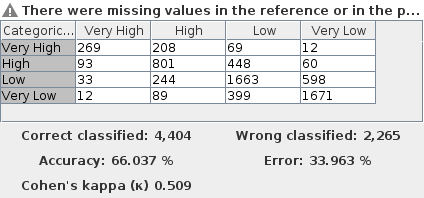
\includegraphics[width=1.1\textwidth]{priceClassificationTraining/DecisionTree}
	\caption{Matrica konfuzije za trening skup za klasifikaciju sa klasifikatorom Decision Tree}
\end{figure}
\newline
\begin{figure}[h!]
	\centering
	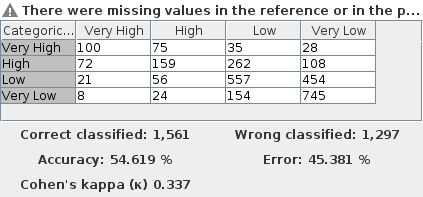
\includegraphics[width=1.1\textwidth]{priceClassificationTest/SVM}
	\caption{Matrica konfuzije za test skup za klasifikaciju sa klasifikatorom SVM}
\end{figure}
\begin{figure}[h!]
	\centering
	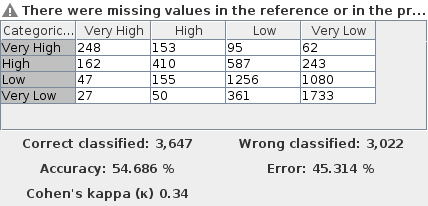
\includegraphics[width=1.1\textwidth]{priceClassificationTraining/SVM}
	\caption{Matrica konfuzije za trening skup za klasifikaciju sa klasifikatorom SVM}
\end{figure}
\newline
\begin{figure}[h!]
	\centering
	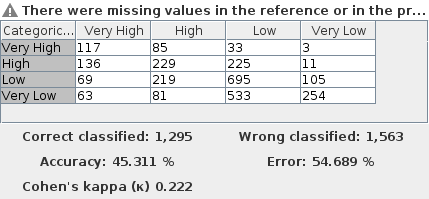
\includegraphics[width=1.1\textwidth]{priceClassificationTest/NaiveBayes}
	\caption{Matrica konfuzije za test skup za klasifikaciju sa klasifikatorom Naive Bayes}
\end{figure}
\begin{figure}[h!]
	\centering
	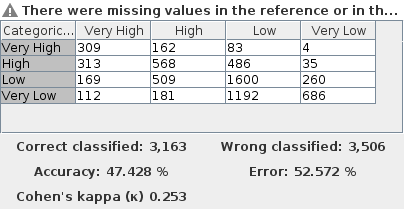
\includegraphics[width=1.1\textwidth]{priceClassificationTraining/NaiveBayes}
	\caption{Matrica konfuzije za trening skup za klasifikaciju sa klasifikatorom Naive Bayes}
\end{figure}
\newline
\begin{figure}[h!]
	\centering
	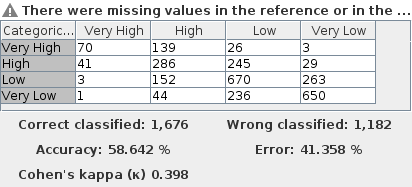
\includegraphics[width=1.1\textwidth]{priceClassificationTest/RProp}
	\caption{Matrica konfuzije za test skup za klasifikaciju sa klasifikatorom RProp MLP}
\end{figure}
\begin{figure}[h!]
	\centering
	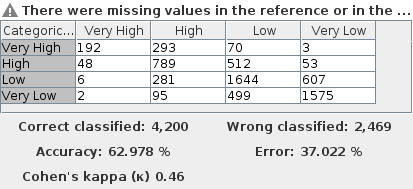
\includegraphics[width=1.1\textwidth]{priceClassificationTraining/RProp}
	\caption{Matrica konfuzije za trening skup za klasifikaciju sa klasifikatorom RProp MLP}
\end{figure}

\end{document}








